% =====================================================================
%  FoodGenome AI - Project Proposal
%  East Delta University
%
%  Build:  tectonic docs/proposal/proposal.tex
%     or:  pdflatex docs/proposal/proposal.tex   (run twice for the ToC)
% =====================================================================

\documentclass[12pt,a4paper,oneside]{report}

% ---------------------------------------------------------------------
%  >>> EDIT THESE FOUR LINES BEFORE SUBMITTING <<<
% ---------------------------------------------------------------------
\newcommand{\StudentName}{A K M Asifuzzaman}
\newcommand{\StudentID}{000000000}          % <-- replace with your real student ID
\newcommand{\CourseCode}{CSE 450 Python Project}
\newcommand{\Instructor}{Arshiana Shamir}
\newcommand{\InstructorTitle}{Lecturer, Department of Computer Science \& Engineering}
\newcommand{\SubmissionDate}{August 1, 2026}
% ---------------------------------------------------------------------

\usepackage[T1]{fontenc}
\usepackage[utf8]{inputenc}
\usepackage{lmodern}
\usepackage{microtype}
\usepackage[a4paper,margin=1.1in]{geometry}
\usepackage{graphicx}
\usepackage{xcolor}
\usepackage{booktabs}
\usepackage{array}
\usepackage{enumitem}
\usepackage{titlesec}
\usepackage{tikz}
\usetikzlibrary{shapes.geometric, arrows.meta, positioning, calc, fit, backgrounds}
\usepackage[hidelinks]{hyperref}

\definecolor{edumaroon}{RGB}{128,20,40}
\definecolor{inkgrey}{RGB}{70,70,70}
\definecolor{panelgrey}{RGB}{244,244,246}

\titleformat{\chapter}[display]
  {\normalfont\Huge\bfseries}{}{0pt}{\Huge}
\titlespacing*{\chapter}{0pt}{-30pt}{24pt}

\setlist[itemize]{leftmargin=1.4em, itemsep=2pt, topsep=4pt}
\setlist[enumerate]{leftmargin=1.6em, itemsep=2pt, topsep=4pt}

\renewcommand{\arraystretch}{1.25}
\linespread{1.10}

\begin{document}

% =====================================================================
%  TITLE PAGE
% =====================================================================
\begin{titlepage}
\centering
\vspace*{1.2cm}

{\LARGE\bfseries EAST DELTA UNIVERSITY\par}

\vspace{1.6cm}

\includegraphics[width=0.30\textwidth]{assets/edu-logo.png}

\vspace{1.6cm}
{\large Title\par}
\vspace{0.35cm}
{\Large\bfseries FOODGENOME AI\par}
\vspace{0.15cm}
{\large\bfseries A Calibrated Multi-Backbone Food Recognition System\\[2pt]
with Retrieval-Augmented Nutritional Reasoning\par}

\vspace{1.4cm}
{\large Presented To\par}
\vspace{0.25cm}
{\large\bfseries \Instructor\par}
{\InstructorTitle\par}

\vspace{1.1cm}
{\large Course\par}
\vspace{0.25cm}
{\large\bfseries \CourseCode\par}

\vspace{1.1cm}
{\large Prepared By\par}
\vspace{0.25cm}
{\large\bfseries \StudentName\par}
{Student ID: \textbf{\StudentID}\par}

\vspace{1.4cm}
{Submitted On: \textbf{\SubmissionDate}\par}

\vfill
\end{titlepage}

% =====================================================================
%  TITLE
% =====================================================================
\chapter*{Title}
\addcontentsline{toc}{chapter}{Title}

\noindent\textbf{\large FoodGenome AI: A Calibrated Multi-Backbone Food Recognition
System with Retrieval-Augmented Nutritional Reasoning}

\vspace{0.8em}
\noindent An end-to-end system that recognises 101 food categories from a single
photograph, reports how confident it is in a statistically meaningful way,
refuses to answer when the photograph is not food, and grounds every nutritional
statement it makes in the United States Department of Agriculture's published
food-composition data.

\newpage
\tableofcontents

% =====================================================================
%  ABSTRACT
% =====================================================================
\chapter*{Abstract}
\addcontentsline{toc}{chapter}{Abstract}

This project proposes FoodGenome AI, an end-to-end food recognition and
nutritional reasoning system built on the Food-101 dataset of 101{,}000
photographs across 101 categories. Rather than training a single classifier,
the system constructs a \emph{frozen feature bank} by caching the embeddings of
three complementary pretrained vision backbones --- SigLIP-SO400M, DINOv2-L and
EVA-02-L --- which reduces every downstream experiment from hours to seconds and
makes rigorous ablation affordable on a single laptop. Lightweight probe
classifiers trained on this bank establish a strong baseline, after which
EVA-02-L is fully fine-tuned at $448\times448$ resolution using layer-wise
learning-rate decay, mixup, CutMix and an exponential moving average of weights.
The final prediction is an ensemble with test-time augmentation, evaluated once
on a test split that is held untouched throughout development.

The central argument of this proposal is that classification accuracy alone is
an insufficient goal for a nutrition application. A confidently wrong calorie
estimate is worse than no estimate at all. FoodGenome AI therefore treats
\emph{reliability} as a first-class deliverable: model confidence is calibrated,
conformal prediction produces prediction sets with a guaranteed coverage rate,
and an out-of-distribution detector rejects photographs that are not food.
Predictions are explained with Grad-CAM and attention maps, and portion size is
estimated from monocular depth. Nutritional answers are produced by a
purpose-built retrieval-augmented generation pipeline --- hybrid sparse and
dense search, reciprocal rank fusion, cross-encoder reranking, corrective
retrieval, explicit grounding and a graph-structured knowledge base derived from
USDA SR Legacy --- so that every figure the system reports is traceable to a
source record. The trained models are exported to ONNX and published on the
Hugging Face Hub, served through a containerised FastAPI backend, and consumed
by a Next.js web application. The target is 96\% top-1 accuracy on Food-101 with
calibrated, auditable and explainable predictions.

% =====================================================================
%  INTRODUCTION
% =====================================================================
\chapter{Introduction}

Dietary self-monitoring is one of the few interventions with consistent evidence
behind it across weight management, diabetes control and cardiovascular health.
Its weakness is not efficacy but adherence. Conventional food logging requires a
person to identify a dish, search a database, choose among near-identical
entries and estimate a portion --- perhaps a dozen interactions for a single
meal, repeated several times a day. Adherence collapses within weeks, and the
tool stops producing value precisely when sustained use would matter most.

A photograph is a far more natural interface. The user points a camera at a
plate; the system does the identification, the database lookup and the portion
estimate. This reframes the problem as fine-grained visual classification
followed by structured knowledge retrieval, and both halves are now tractable.
Vision transformers pretrained on web-scale corpora transfer remarkably well to
food imagery, and retrieval-augmented generation allows a language model to
answer nutritional questions from an authoritative database instead of from
memorised parameters.

Food classification is nonetheless a genuinely difficult fine-grained problem.
The Food-101 categories include pairs that differ only in ingredients invisible
from above --- spaghetti bolognese against spaghetti carbonara, filet mignon
against prime rib, beef carpaccio against beef tartare. Intra-class variation is
extreme: the dataset is deliberately built from unretouched user photographs,
so lighting, plating, camera angle and cuisine-specific presentation vary
enormously within every class. The training split is also known to contain a
degree of label noise, which the original authors left in place intentionally.

This project treats the visual problem seriously, but argues that solving it is
only half the work. A nutrition system that answers every query with equal
confidence, that has no mechanism for saying ``this is not food'' or ``I am not
sure between these three dishes'', and that cannot show where its numbers came
from, is not safe to put in front of a user regardless of its headline accuracy.
The proposed system is therefore organised around accuracy, reliability,
explainability and grounding as four co-equal objectives.

% =====================================================================
%  BACKGROUND
% =====================================================================
\chapter{Background}

\section{Transfer learning and modern vision backbones}

The dominant paradigm in image classification is to adapt a model pretrained on
a very large corpus rather than to train from scratch. Three families of
pretraining are relevant here, and they fail in different ways, which is exactly
why combining them is productive:

\begin{itemize}
  \item \textbf{Language-supervised contrastive models.} SigLIP is trained to
  align images with their captions using a pairwise sigmoid loss. Because
  captions name dishes, the resulting features carry strong semantic priors
  about food categories.
  \item \textbf{Self-supervised models.} DINOv2 is trained without labels or
  text through self-distillation. Its features are sensitive to texture, surface
  and part structure --- properties that distinguish a seared crust from a
  braised one --- and are statistically decorrelated from contrastive features.
  \item \textbf{Supervised fine-grained models.} EVA-02 combines masked image
  modelling with supervised fine-tuning on ImageNet-22k, giving it a strong
  prior for exactly the kind of fine-grained discrimination Food-101 demands.
\end{itemize}

Because these three make different mistakes, an ensemble over them recovers
accuracy that no single backbone achieves alone.

\section{Frozen features as an experimental strategy}

Fine-tuning a 300M-parameter backbone on consumer hardware costs hours per
experiment, which in practice limits a student project to a handful of
configurations chosen largely by guesswork. Running each backbone over the
corpus exactly once and caching the pooled embeddings converts every subsequent
experiment --- head architecture, calibration method, conformal score,
out-of-distribution rule, ensemble weighting --- into a computation that
finishes in seconds. The cache is what makes a rigorous, ablation-driven study
feasible within the constraints of this course.

\section{Calibration, conformal prediction and OOD detection}

Modern neural networks are systematically overconfident: a softmax output of
0.95 does not correspond to being correct 95\% of the time. Temperature scaling
corrects this with a single parameter fitted on held-out data. Conformal
prediction goes further and returns a \emph{set} of labels guaranteed, under an
exchangeability assumption, to contain the true label at a chosen rate --- so
the system can honestly report ``this is one of these three dishes'' instead of
guessing. Separately, any classifier restricted to 101 categories will
confidently assign one of them to a photograph of a keyboard; an
out-of-distribution detector is required for the system to decline.

\section{Retrieval-augmented generation}

RAG grounds a language model's output in retrieved documents rather than its
parameters. A production-grade pipeline requires considerably more than a single
vector search: sparse and dense retrieval capture different query intents and
must be fused; a cross-encoder reranker is needed because bi-encoder similarity
is a weak relevance signal; corrective retrieval detects and repairs low-quality
retrievals before generation; and grounding verification checks that generated
claims are actually supported by the retrieved evidence. For a nutrition
assistant, where a hallucinated figure is a safety issue, these are requirements
rather than refinements.

% =====================================================================
%  PROBLEM STATEMENT
% =====================================================================
\chapter{Problem Statement}

Existing photograph-based food recognition applications share a set of
structural weaknesses:

\begin{enumerate}
  \item \textbf{They emit point predictions without honest uncertainty.} A
  single label is returned with an uncalibrated confidence score. The user
  cannot distinguish a near-certain identification from a coin flip between two
  visually similar dishes.
  \item \textbf{They cannot decline.} Presented with a photograph that contains
  no food, a 101-way classifier still returns one of its 101 categories, often
  with high confidence.
  \item \textbf{Their nutritional figures are unsourced.} Numbers appear without
  provenance, and where a language model is involved they may be fabricated
  outright. In a health context this is not a cosmetic problem.
  \item \textbf{They are opaque.} No indication is given of which region of the
  image drove the decision, leaving the user with no means of noticing an error.
  \item \textbf{Portion size is ignored.} Nutritional data is published per
  100\,g, so a per-100\,g figure presented as a per-serving figure can be wrong
  by a factor of three or more.
\end{enumerate}

A preliminary experiment conducted during the preparation of this proposal
illustrates how severe the grounding problem is in practice. Matching the 101
Food-101 category names against USDA SR Legacy by naive text search produced
confidently incorrect results for a large fraction of classes: \textit{beef
carpaccio} resolved to ``Soup, stock, beef'' at 13\,kcal per 100\,g,
\textit{chicken wings} to ``Soup, stock, chicken'' at 36\,kcal, \textit{filet
mignon} to a salmon product, and \textit{chocolate cake} to a snack cake
explicitly labelled ``not chocolate''. Roughly a quarter of the categories
matched no meaningful record at all. Any system that adopts such a mapping
without curation will present users with calorie figures that are wrong by an
order of magnitude while appearing entirely authoritative. This finding directly
motivates the curated, auditable knowledge base described in
Chapter~\ref{ch:methodology}.

\medskip
\noindent This project therefore addresses the following question: \emph{can a
food recognition system be built on consumer hardware that is simultaneously
highly accurate, statistically calibrated, capable of abstaining, visually
explainable, and grounded in an auditable nutritional source?}

% =====================================================================
%  OBJECTIVES
% =====================================================================
\chapter{Objectives}

\begin{enumerate}
  \item Build a cached multi-backbone feature bank over Food-101 to make
  systematic experimentation computationally feasible.
  \item Achieve 96\% top-1 accuracy on the Food-101 test split through
  fine-tuning and ensembling, measured once under a protocol that prevents
  optimistic bias.
  \item Calibrate predicted confidence and quantify the improvement with
  expected calibration error.
  \item Produce conformal prediction sets with an empirically verified coverage
  guarantee.
  \item Implement an out-of-distribution detector that rejects non-food imagery
  at a measured false-positive rate.
  \item Generate visual explanations for every prediction, and estimate portion
  mass from monocular depth.
  \item Construct a curated, fully auditable nutritional knowledge base covering
  all 101 categories, sourced from USDA SR Legacy.
  \item Implement an advanced retrieval pipeline with hybrid search, reciprocal
  rank fusion, reranking, corrective retrieval, grounding verification and a
  graph-structured knowledge representation.
  \item Evaluate that pipeline against a hand-curated gold-standard question set
  using standard retrieval and generation metrics.
  \item Deliver the system as a deployed, publicly accessible web application
  with published model artefacts and reproducible training notebooks.
\end{enumerate}

% =====================================================================
%  METHODOLOGY
% =====================================================================
\chapter{Proposed Methodology}
\label{ch:methodology}

The work is organised into four phases and fourteen stages.

\section{Phase A --- Perception}

\textbf{Stage 1: Frozen feature bank.} Each of the three backbones is run
exactly once over all 101{,}000 images and the pooled embeddings are cached to
disk as half-precision arrays.

\textbf{Stage 2: Classification heads.} Probe classifiers are trained on the
cached features. Because the embedding spaces of the three backbones are scaled
differently, a \emph{gated fusion} head is used: each backbone is projected to a
common width and a learned gate weighs them per sample. The gate values are
themselves interpretable, showing which backbone the model relies on for which
foods.

\textbf{Stage 3: Fine-tuning.} EVA-02-L is fully fine-tuned at $448\times448$
with layer-wise learning-rate decay, mixup and CutMix, label smoothing, stochastic
depth, cosine scheduling with warmup, and an exponential moving average of
weights.

\textbf{Stage 4: Ensemble and evaluation.} The fine-tuned model and the fusion
head are combined with test-time augmentation, and the result is evaluated once
on the untouched test split.

\section{Phase B --- Reliability}

\textbf{Stage 5: Calibration, conformal prediction and OOD detection.}
Temperature and vector scaling are fitted on the validation split and assessed
by expected calibration error. Adaptive prediction sets are constructed to
achieve a target coverage level. An out-of-distribution detector combining
energy-based scoring with Mahalanobis distance in feature space rejects non-food
images.

\textbf{Stage 6: Explainability and portion estimation.} Grad-CAM and attention
rollout produce per-prediction visual explanations. Monocular depth estimation
combined with the segmented food region yields a volume proxy, converted to mass
using per-category density priors.

\section{Phase C --- Knowledge and retrieval}

\textbf{Stage 7: Nutrition knowledge base.} A curated mapping is built from each
of the 101 categories to USDA SR Legacy. Where SR Legacy contains the dish, a
specific record is pinned; where it does not --- roughly thirty categories,
including tiramisu, bibimbap and takoyaki --- the dish is represented as a
weighted composite of ingredient records, which additionally supplies the
dish-to-ingredient edges used in Stage 8. Every entry is auditable back to its
source records.

\textbf{Stage 8: Advanced RAG pipeline.} Sparse BM25 and dense embedding
retrieval are fused by reciprocal rank fusion, reranked by a cross-encoder,
checked and repaired by corrective retrieval, verified for grounding, and
augmented by a graph representation linking dishes, ingredients and nutrients.
Generation is performed by an OpenAI model behind a provider-agnostic interface;
all retrieval components run locally.

\textbf{Stage 9: RAG evaluation.} A hand-curated gold-standard question set is
used to measure retrieval quality (recall@$k$, MRR, nDCG) and generation quality
(faithfulness, answer relevance, context precision and recall).

\section{Phase D --- Delivery}

\textbf{Stages 10--14.} Models are exported to ONNX and published to the Hugging
Face Hub; a FastAPI backend is containerised for Hugging Face Spaces; a Next.js
front end is built on a bespoke comic-inspired design system; training notebooks,
architecture documentation, an illustrated README, a written report and slides
are produced; and the complete system is deployed.

% =====================================================================
%  ARCHITECTURE
% =====================================================================
\chapter{System Architecture}

\begin{figure}[h]
\centering
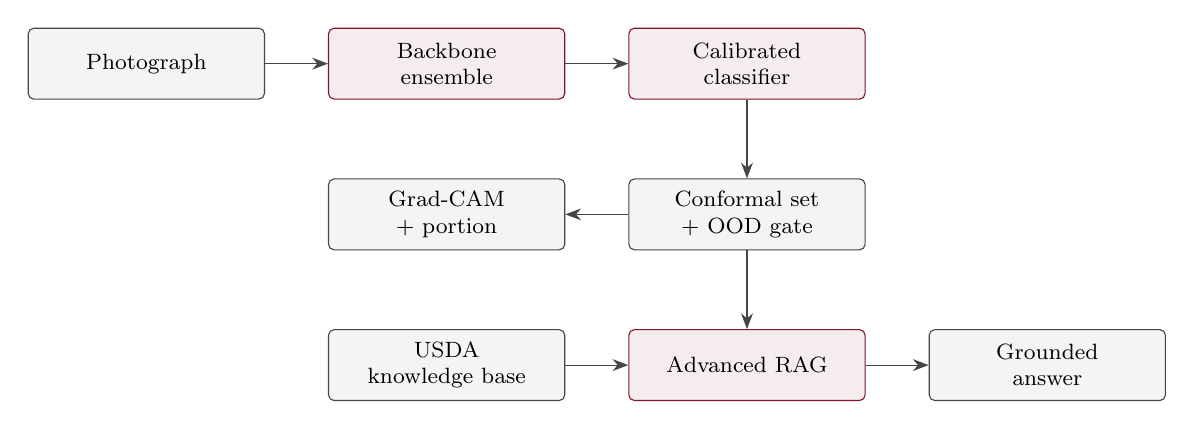
\begin{tikzpicture}[
  node distance=8mm,
  box/.style={rectangle, rounded corners=2pt, draw=inkgrey, fill=panelgrey,
              minimum width=30mm, minimum height=9mm, align=center,
              font=\footnotesize},
  accent/.style={box, draw=edumaroon, fill=edumaroon!8},
  arrow/.style={-{Stealth[length=2mm]}, draw=inkgrey}
]
\node[box] (img) {Photograph};
\node[accent, right=of img] (bb) {Backbone\\ensemble};
\node[accent, right=of bb] (head) {Calibrated\\classifier};
\node[box, below=10mm of head] (conf) {Conformal set\\+ OOD gate};
\node[box, left=of conf] (xai) {Grad-CAM\\+ portion};
\node[accent, below=10mm of conf] (rag) {Advanced RAG};
\node[box, left=of rag] (kb) {USDA\\knowledge base};
\node[box, right=of rag] (out) {Grounded\\answer};

\draw[arrow] (img) -- (bb);
\draw[arrow] (bb) -- (head);
\draw[arrow] (head) -- (conf);
\draw[arrow] (conf) -- (xai);
\draw[arrow] (conf) -- (rag);
\draw[arrow] (kb) -- (rag);
\draw[arrow] (rag) -- (out);
\end{tikzpicture}
\caption{End-to-end flow. A photograph is embedded by the backbone ensemble,
classified by a calibrated head, gated by conformal and out-of-distribution
checks, explained visually, and finally answered against the curated knowledge
base through the retrieval pipeline.}
\end{figure}

% =====================================================================
%  DATASET
% =====================================================================
\chapter{Dataset and Experimental Setup}

\section{Food-101}

Food-101 contains 101 categories with 1{,}000 images each. The official split
provides 750 training and 250 test images per class.

\begin{table}[h]
\centering
\begin{tabular}{lr}
\toprule
\textbf{Property} & \textbf{Value} \\
\midrule
Categories & 101 \\
Training images & 75{,}750 \\
Test images & 25{,}250 \\
Total images & 101{,}000 \\
On-disk size & 6.1\,GB \\
\bottomrule
\end{tabular}
\caption{Food-101 as downloaded and verified locally.}
\end{table}

Food-101 ships only a training and a test split. Reporting model-selection
results on the test split is the single most common way projects of this kind
overstate their accuracy. A fixed, class-stratified 4\% validation slice is
therefore carved out of the training split under a fixed random seed and shared
by both the image and the cached-feature pipelines, and \textbf{the test split is
not consulted until final evaluation}.

\section{USDA SR Legacy}

Nutritional data is taken from USDA FoodData Central's SR Legacy release, the
last USDA release providing complete micronutrient profiles for generic,
unbranded foods --- the correct reference when the input is a dish rather than a
packaged product. Thirty-two nutrients per food are tracked, along with
published portion weights.

\section{Hardware and measured throughput}

All training is performed locally on an Apple M3 Pro with 18\,GB of unified
memory using PyTorch's Metal backend. The following throughput figures were
measured directly rather than estimated.

\begin{table}[h]
\centering
\begin{tabular}{lrrrr}
\toprule
\textbf{Backbone} & \textbf{Res.} & \textbf{Params} & \textbf{Throughput} & \textbf{Full corpus} \\
\midrule
SigLIP-SO400M & 384 & 428.2M & 5.3 img/s & $\sim$316 min \\
EVA-02-L      & 448 & 304.1M & 4.1 img/s & $\sim$414 min \\
DINOv2-L      & 518 & 304.4M & 3.6 img/s & $\sim$464 min \\
\bottomrule
\end{tabular}
\caption{Measured inference throughput at batch size 8 in half precision. The
one-off cost of building the feature bank is approximately 20 hours; every
experiment afterwards runs against the cache in seconds.}
\end{table}

% =====================================================================
%  EVALUATION
% =====================================================================
\chapter{Evaluation Plan}

\begin{table}[h]
\centering
\begin{tabular}{p{4.2cm}p{9.2cm}}
\toprule
\textbf{Dimension} & \textbf{Metrics} \\
\midrule
Classification & Top-1 and top-5 accuracy, macro-F1, per-class accuracy,
confusion analysis of the hardest pairs \\
Calibration & Expected and maximum calibration error, reliability diagrams,
Brier score \\
Conformal prediction & Empirical coverage against the target level, average
prediction-set size \\
OOD detection & AUROC and FPR at 95\% true-positive rate against non-food
imagery \\
Portion estimation & Mean absolute percentage error against a hand-measured
reference set \\
Retrieval & Recall@$k$, MRR, nDCG on the gold-standard question set \\
Generation & Faithfulness, answer relevance, context precision and recall \\
System & End-to-end latency, model size, cold-start time \\
\bottomrule
\end{tabular}
\caption{Evaluation dimensions and the metrics reported for each.}
\end{table}

Reported accuracy will be compared against published Food-101 results to
establish where the system sits relative to the literature. All numbers will be
produced by scripts committed to the repository so that they can be regenerated.

% =====================================================================
%  OUTCOMES
% =====================================================================
\chapter{Expected Outcomes}

\begin{itemize}
  \item A Food-101 classifier reaching approximately 96\% top-1 accuracy,
  measured under a protocol that prevents test-set leakage.
  \item Calibrated confidence estimates and conformal prediction sets with a
  verified coverage guarantee.
  \item A working out-of-distribution rejector for non-food photographs.
  \item Visual explanations and depth-based portion estimates for every
  prediction.
  \item A curated, auditable nutritional knowledge base covering all 101
  categories.
  \item An advanced retrieval pipeline with a measured evaluation against a
  hand-built gold standard.
  \item Public artefacts: models on the Hugging Face Hub, a containerised API on
  Hugging Face Spaces, a deployed web application, and a documented open-source
  repository with notebooks covering every training stage.
\end{itemize}

% =====================================================================
%  TOOLS
% =====================================================================
\chapter{Tools and Technologies}

\begin{table}[h]
\centering
\begin{tabular}{p{3.6cm}p{9.8cm}}
\toprule
\textbf{Area} & \textbf{Technology} \\
\midrule
Language & Python 3.11 \\
Deep learning & PyTorch 2.13 (Metal backend), timm, Hugging Face Transformers \\
Data & Hugging Face Datasets, NumPy, pandas, Pillow \\
Retrieval & sentence-transformers, FAISS, BM25, cross-encoder reranking \\
Generation & OpenAI API behind a provider-agnostic interface \\
Backend & FastAPI, ONNX Runtime, Docker, Hugging Face Spaces \\
Frontend & Next.js, TypeScript, Vercel \\
Reporting & Jupyter, Matplotlib, \LaTeX, Mermaid \\
\bottomrule
\end{tabular}
\end{table}

% =====================================================================
%  TIMELINE
% =====================================================================
\chapter{Timeline}

\begin{table}[h]
\centering
\begin{tabular}{clp{7.4cm}}
\toprule
\textbf{Week} & \textbf{Phase} & \textbf{Deliverable} \\
\midrule
1 & A & Feature bank complete; probe heads and fusion ensemble trained \\
2 & A & EVA-02-L fine-tuned at 448; ensemble with TTA; final test evaluation \\
3 & B & Calibration, conformal prediction, OOD detection, Grad-CAM, portion
estimation \\
4 & C & Curated nutrition knowledge base for all 101 categories \\
5 & C & Advanced RAG pipeline and its gold-standard evaluation \\
6 & D & ONNX export, Hub publication, FastAPI backend, Docker image \\
7 & D & Next.js front end and deployment \\
8 & D & Notebooks, documentation, report and slides \\
\bottomrule
\end{tabular}
\end{table}

% =====================================================================
%  REFERENCES
% =====================================================================
\chapter*{References}
\addcontentsline{toc}{chapter}{References}

\begin{enumerate}[leftmargin=*, itemsep=4pt]
  \item L.~Bossard, M.~Guillaumin and L.~Van Gool. Food-101 --- Mining
  Discriminative Components with Random Forests. \emph{ECCV}, 2014.
  \item X.~Zhai, B.~Mustafa, A.~Kolesnikov and L.~Beyer. Sigmoid Loss for
  Language Image Pre-Training. \emph{ICCV}, 2023.
  \item M.~Oquab et al. DINOv2: Learning Robust Visual Features without
  Supervision. \emph{TMLR}, 2024.
  \item Y.~Fang et al. EVA-02: A Visual Representation for Neon Genesis.
  \emph{arXiv:2303.11331}, 2023.
  \item C.~Guo, G.~Pleiss, Y.~Sun and K.~Q.~Weinberger. On Calibration of Modern
  Neural Networks. \emph{ICML}, 2017.
  \item A.~N.~Angelopoulos and S.~Bates. A Gentle Introduction to Conformal
  Prediction and Distribution-Free Uncertainty Quantification.
  \emph{arXiv:2107.07511}, 2021.
  \item D.~Hendrycks and K.~Gimpel. A Baseline for Detecting Misclassified and
  Out-of-Distribution Examples in Neural Networks. \emph{ICLR}, 2017.
  \item R.~R.~Selvaraju et al. Grad-CAM: Visual Explanations from Deep Networks
  via Gradient-Based Localization. \emph{ICCV}, 2017.
  \item P.~Lewis et al. Retrieval-Augmented Generation for Knowledge-Intensive
  NLP Tasks. \emph{NeurIPS}, 2020.
  \item G.~V.~Cormack, C.~L.~A.~Clarke and S.~Buettcher. Reciprocal Rank Fusion
  Outperforms Condorcet and Individual Rank Learning Methods. \emph{SIGIR}, 2009.
  \item S.-Q.~Yan et al. Corrective Retrieval Augmented Generation.
  \emph{arXiv:2401.15884}, 2024.
  \item D.~Edge et al. From Local to Global: A Graph RAG Approach to
  Query-Focused Summarization. \emph{arXiv:2404.16130}, 2024.
  \item I.~Loshchilov and F.~Hutter. Decoupled Weight Decay Regularization.
  \emph{ICLR}, 2019.
  \item H.~Zhang, M.~Cisse, Y.~N.~Dauphin and D.~Lopez-Paz. mixup: Beyond
  Empirical Risk Minimization. \emph{ICLR}, 2018.
  \item S.~Yun et al. CutMix: Regularization Strategy to Train Strong
  Classifiers with Localizable Features. \emph{ICCV}, 2019.
  \item U.S. Department of Agriculture, Agricultural Research Service.
  \emph{FoodData Central: SR Legacy}. 2018.
\end{enumerate}

\end{document}
